\documentclass{article}

\usepackage{amsmath, amssymb, amsfonts}
\usepackage[margin=1in]{geometry}
\usepackage{graphicx}

\begin{document}
	The Navier-Stokes energy density evolution equation I used, as I found in the literature is 
	\begin{equation}
		\partial_\tau \epsilon + \frac{\epsilon + p}{\tau} - \eta\frac{4}{3\tau^2} = 0
	\end{equation}
	Using that $p = \epsilon/3$ and the relation $\epsilon + p = sT$, I rewrote the equation as 
	\begin{equation}
		\partial_\tau \epsilon + \frac{4}{3\tau}\epsilon\left(1-\frac{\eta}{sT}\frac{4}{3\tau}\right)= 0
	\end{equation}
	Lastly, using the relaxation time $\tau_\mathrm{r} = 5\eta/sT$, we have
	\begin{equation}
		\partial_\tau +\frac{4}{3\tau}\epsilon\left(1-\frac{4}{15}\frac{\tau_\mathrm{r}}{\tau}\right) = 0
	\end{equation}
	Using the inital conditions $T_0 = 0.60$ GeV and $\tau_0 = 0.25$ fm/c and $\eta = 1/4\pi$, the energy evolution that I calculate is 
	\begin{figure}[h]
		\centering
		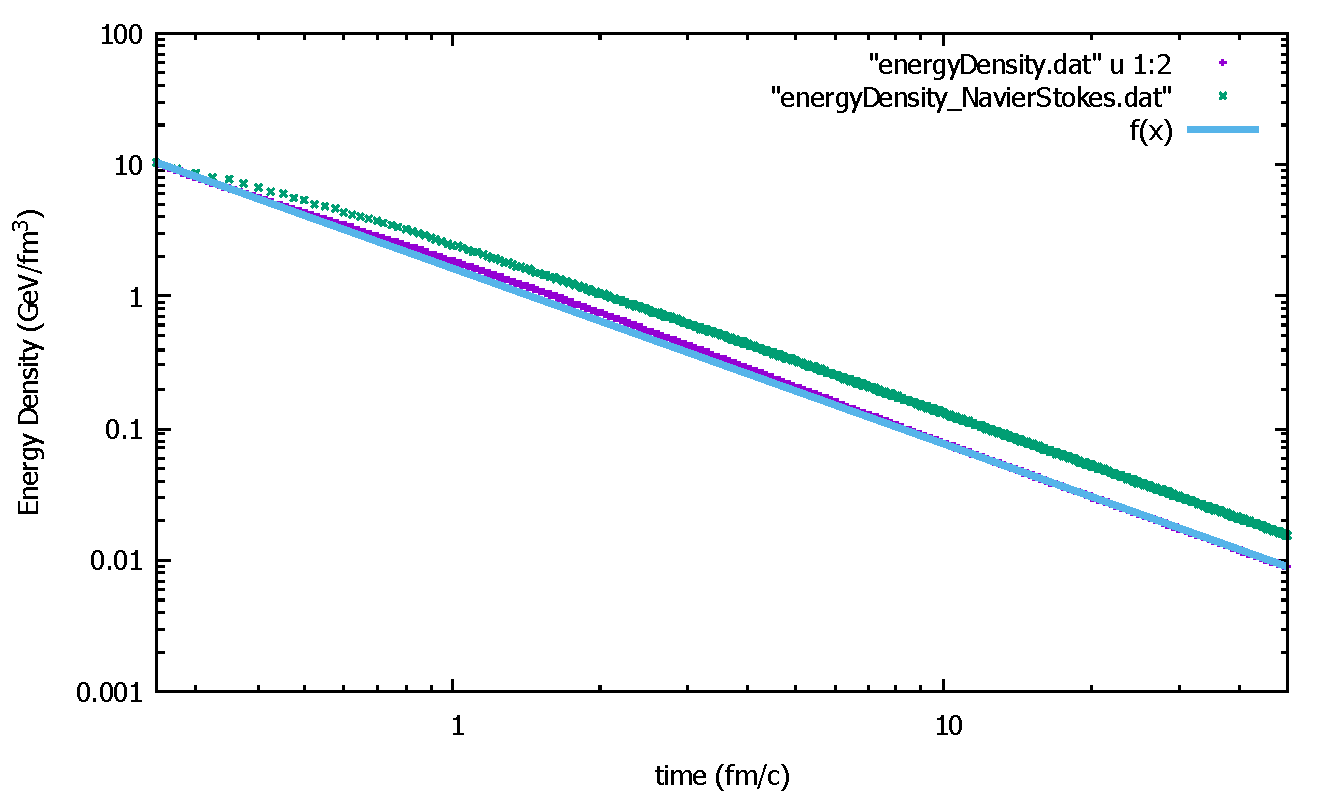
\includegraphics[width=.85\textwidth]{Navier-Stokes.pdf}
		\caption{The purple data points are the energy evolution as calculated by Strickland's code with the same inital conditions, the green is the Navier-Stokes data, and the blue line is the the equation $\epsilon = 6C\tau^{-4/3}/(\pi^2\hbar^3c^3)$}
	\end{figure}
	
\end{document}